\documentclass[journal]{IEEEtran}

\usepackage{cite}
\usepackage{amsmath,amssymb}
\usepackage{graphicx}
\usepackage{booktabs}
\usepackage[hidelinks]{hyperref}
\usepackage{orcidlink}
\usepackage{url}

\graphicspath{{../outputs/figures_final/}{../outputs/figures/}}
\newcommand{\sigmarun}{0.0053}
\newcommand{\rEpochTest}{0.49}
\newcommand{\rValTest}{0.004}
\newcommand{\meanDeltaEpoch}{11.3}
\newcommand{\dTestClose}{0.0044}
\newcommand{\dTestFar}{0.0108}
\newcommand{\nPairs}{47}
\newcommand{\detSmallLo}{0.44}
\newcommand{\detSmallHi}{0.59}
\newcommand{\diceSmallLo}{0.40}
\newcommand{\diceSmallHi}{0.53}
\newcommand{\detLargeLo}{0.86}
\newcommand{\detLargeHi}{0.89}
\newcommand{\nSmallExt}{123}
\newcommand{\nSmallKvasir}{6}
\newcommand{\pctSmallEtis}{31.6}
\newcommand{\pctSmallKvasir}{0.6}
\newcommand{\sesGapLo}{0.055}
\newcommand{\sesGapHi}{0.078}
\newcommand{\nBelowNoise}{4}
\newcommand{\nPairsTotal}{10}
\newcommand{\sigmaInDomain}{3.9}
\newcommand{\sigmaEtis}{21.6}
\newcommand{\ttaIn}{0.0050}
\newcommand{\ttaOut}{0.0107}
\newcommand{\bestInDomain}{SegFormer-B2}
\newcommand{\bestInDomainDice}{0.9142}
\newcommand{\worstEtis}{0.6551}
\newcommand{\bestEtis}{0.7706}
\newcommand{\kvasirMedianArea}{11.4}
\newcommand{\nQualSmall}{123}
\newcommand{\nQualAllMiss}{44}
\newcommand{\pctQualAllMiss}{36}
\newcommand{\nQualZeroDice}{16}


\begin{document}

\title{What Polyp Segmentation Benchmarks Cannot Measure:\\
Small Lesions, Domain Shift, and a Noise Floor\\
Larger Than Most Reported Gains}

\author{Rishit~Puri~\orcidlink{0009-0004-6215-9997}%
\thanks{R.~Puri is a software engineer at Karl Storz Endoscopy
(e-mail: rishitpuri15@gmail.com; \mbox{ORCID} 0009-0004-6215-9997).
This work was carried out independently of his employment; see the competing
interests statement.}}

\maketitle


\begin{abstract}
Automated polyp segmentation is almost universally benchmarked as a single
mean Dice score on one train/test split of Kvasir-SEG, where reported values
now cluster within a few points of one another. We ask what that protocol can
and cannot measure. Training five architectures spanning four backbone
families under one recipe, with five-fold cross-validation over all 1000
Kvasir-SEG images and zero-shot transfer to four external datasets (1248 images), we report three findings. First, on lesions occupying less than 1\%
of the image---the clinically small polyps that are missed most often in
practice---per-lesion detection falls to \detSmallLo--\detSmallHi\ from
\detLargeLo--\detLargeHi\ for larger lesions: models miss roughly half of
them. Kvasir-SEG contains \nSmallKvasir\ such images out of 1000, so this
failure is nearly invisible to in-domain benchmarking. Second, by repeating
identical training configurations we measure a run-to-run noise floor of
$\sigma_{\mathrm{run}}=\sigmarun$ Dice; \nBelowNoise\ of \nPairsTotal\
pairwise in-domain architecture comparisons fall below it. This variance is
not removed by fixing seeds, by seeding data-loader workers, or by
deterministic CUDA kernels; it arises from checkpoint selection on a flat
validation curve, with identical runs selecting epochs \meanDeltaEpoch\ apart
on average. Third, the resolving power of a test set depends strongly on
domain shift: the same five architectures span \sigmaInDomain$\sigma$
in-domain but \sigmaEtis$\sigma$ on ETIS-Larib. We also document a subgroup
finding of our own that failed to replicate when the single split was
replaced by cross-validation. We release code, splits and per-image results
for all 88 training runs.
\end{abstract}

\begin{IEEEkeywords}
polyp segmentation, colonoscopy, evaluation
methodology, domain shift, reproducibility, medical image analysis
\end{IEEEkeywords}

\section{Introduction}

Colorectal cancer is among the most commonly diagnosed cancers worldwide, and
colonoscopic detection and removal of precursor lesions is the principal
prevention pathway. Tandem-colonoscopy studies nonetheless report polyp miss
rates of 14--30\%, concentrated in small and flat (sessile) lesions that are
poorly distinguished from surrounding mucosa \cite{leufkens2012,vanrijn2006}.
Computer-aided detection is therefore motivated less by average-case accuracy
than by performance on precisely those lesions.

The field's dominant benchmark is Kvasir-SEG \cite{jha2020kvasirseg}: 1000
colonoscopy images with expert segmentation masks. The conventional protocol
reports a single mean Dice score on one held-out split, and published values
now sit in a narrow band. When many methods report scores within a few points
of one another, the question of what the benchmark can actually resolve
becomes as important as the methods themselves.

This paper is a measurement study rather than a proposal for a new
architecture. We ask three questions:

\begin{enumerate}
\item \textbf{Which lesions do current models fail on, and does the benchmark
contain them?} We stratify by true lesion size and by sessile morphology, in
domain and across four external datasets.
\item \textbf{How large is the noise floor?} We repeat identical training
configurations to measure run-to-run variance directly, and ask which
architecture differences exceed it.
\item \textbf{How much does the choice of test set matter?} We compare the
resolving power of in-domain and out-of-domain evaluation.
\end{enumerate}

Our answers are, in brief: models miss about half of clinically small lesions
and the standard benchmark contains almost none of them; the noise floor is
comparable to the differences routinely reported as improvements, and is
caused by checkpoint selection rather than by anything a random seed
controls; and cross-dataset evaluation resolves architectures roughly five
times better than in-domain evaluation. We also report, as a worked example
of the first problem, a subgroup finding from our own single-split analysis
that did not survive cross-validation.

\section{Results}

\subsection{Aggregate in-domain performance is tightly clustered}

Table~\ref{tab:indomain} reports five-fold cross-validated performance on
Kvasir-SEG, in which every image is tested exactly once. The five
architectures span 3.7--28.1M parameters and four backbone families, yet
their Dice scores fall within 0.021 of one another, with
\bestInDomain\ best at \bestInDomainDice. Boundary-F1 and HD95 broadly track
Dice. This clustering is the phenomenon that motivates the rest of the paper:
if architectures differ this little on the standard benchmark, the benchmark's
own precision determines whether those differences mean anything.

\begin{table*}[t]
\centering
\footnotesize
\caption{In-domain performance under five-fold cross-validation on Kvasir-SEG. Every image is tested exactly once ($n=1000$ per model). HD95 is expressed as a percentage of the image diagonal; the detection rate is the fraction of ground-truth lesions matched at IoU $\geq 0.5$.}
\label{tab:indomain}
\begin{tabular}{lrccccc}
\toprule
Model & Par.\ (M) & Dice & IoU & Boundary-F1 & HD95 (\%) & Det.\ rate \\
\midrule
U-Net & 24.4 & 0.9007 & 0.8426 & 0.6725 & 5.89 & 0.9308 \\
U-Net++ & 26.1 & 0.9011 & 0.8437 & 0.6777 & 6.34 & 0.9328 \\
SegFormer-B0 & 3.7 & 0.8932 & 0.8293 & 0.5947 & 6.14 & 0.9269 \\
SegFormer-B2 & 24.7 & \textbf{0.9142} & 0.8598 & 0.6661 & \textbf{4.86} & \textbf{0.9408} \\
U-Net+PVTv2 & 28.1 & 0.9133 & \textbf{0.8606} & \textbf{0.6995} & 5.29 & 0.9334 \\
\bottomrule
\end{tabular}
\end{table*}


\subsection{Models miss about half of clinically small lesions}

Stratifying all 2248 test images by true lesion size gives the paper's
central result (Table~\ref{tab:size}, Fig.~\ref{fig:small}). For lesions
larger than 5\% of the image, per-lesion detection is
\detLargeLo--\detLargeHi. For lesions below 1\%---the size range that
dominates clinical misses---detection collapses to
\detSmallLo--\detSmallHi\ and Dice roughly halves, to
\diceSmallLo--\diceSmallHi. In other words, on the lesions that matter most,
current models fail to find approximately one in two.

\begin{figure*}[t]
\centering
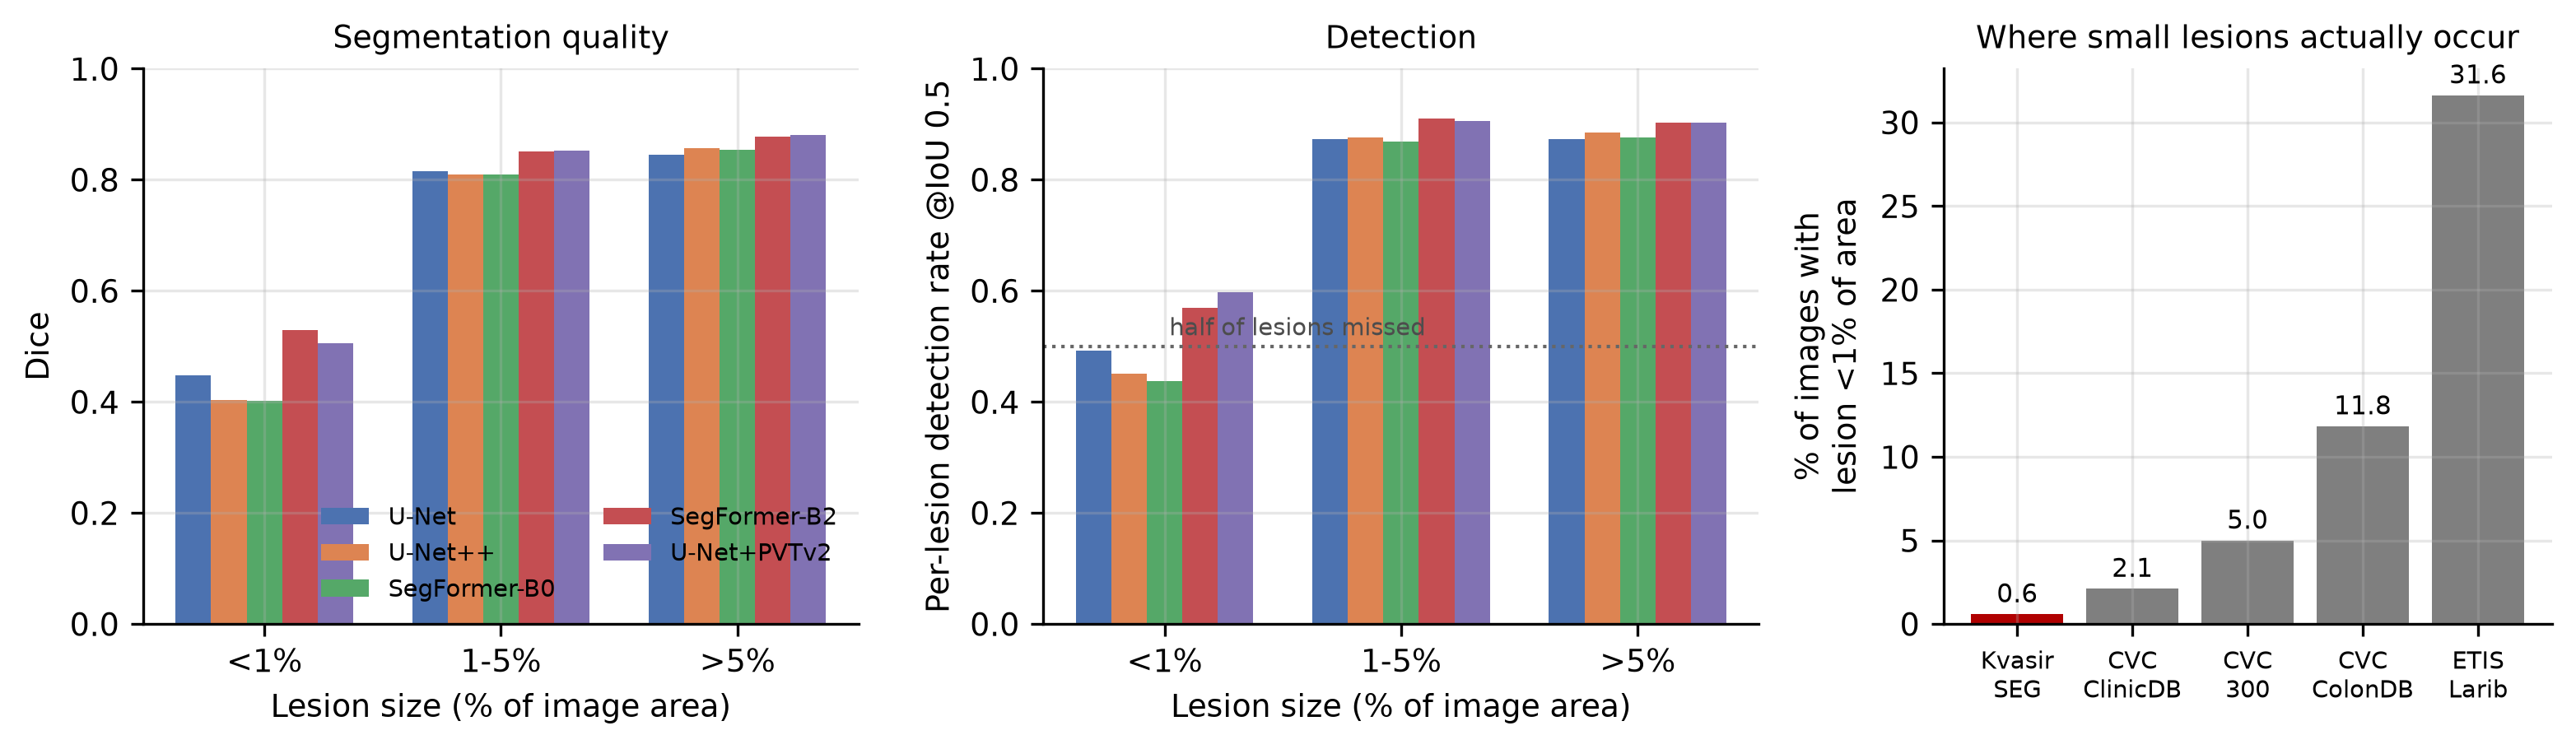
\includegraphics[width=0.92\textwidth]{f1_small_polyp.pdf}
\caption{Performance against true lesion size, pooled over all test images.
Left: Dice. Centre: per-lesion detection rate; the dotted line marks half of
lesions missed. Right: the proportion of images in each dataset whose lesion
occupies less than 1\% of the frame. Kvasir-SEG, the field's primary
benchmark, contains \pctSmallKvasir\% such images against \pctSmallEtis\% for
ETIS-Larib.}
\label{fig:small}
\end{figure*}

\begin{table*}[t]
\centering
\footnotesize
\caption{Performance by true lesion size, pooled over all test images (in-domain and external). Lesions occupying less than 1\% of the image are segmented far worse and, more importantly, are missed outright about half of the time. Kvasir-SEG contains only 6 such images, so this failure mode is nearly invisible to in-domain benchmarking.}
\label{tab:size}
\begin{tabular}{lcccccc}
\toprule
 & \multicolumn{3}{c}{Dice} & \multicolumn{3}{c}{Detection rate} \\
\cmidrule(lr){2-4}\cmidrule(lr){5-7}
Model & $<$1\% & 1--5\% & $>$5\% & $<$1\% & 1--5\% & $>$5\% \\
\midrule
U-Net & 0.4461 & 0.8101 & 0.8289 & 0.489 & 0.869 & 0.857 \\
U-Net++ & 0.4022 & 0.8050 & 0.8415 & 0.449 & 0.873 & 0.870 \\
SegFormer-B0 & 0.4034 & 0.8047 & 0.8403 & 0.437 & 0.865 & 0.862 \\
SegFormer-B2 & 0.5271 & 0.8483 & 0.8656 & 0.566 & 0.908 & 0.892 \\
U-Net+PVTv2 & 0.5026 & 0.8503 & 0.8689 & 0.594 & 0.907 & 0.892 \\
\bottomrule
\end{tabular}
\end{table*}


Crucially, this failure mode is almost absent from the benchmark used to
develop these models. The median Kvasir-SEG lesion occupies
\kvasirMedianArea\% of the frame, and only \nSmallKvasir\ of its 1000 images
contain a lesion below 1\%---compared with \pctSmallEtis\% of ETIS-Larib
(Fig.~\ref{fig:small}, right). Consistent with this, the in-domain
size contrast is weak and inconsistent: comparing the smallest against the
largest Kvasir-SEG size tertile, the difference is statistically
indistinguishable from zero for three of five architectures. The in-domain
``small'' stratum is small only relative to a dataset of large lesions.

\begin{figure*}[t]
\centering
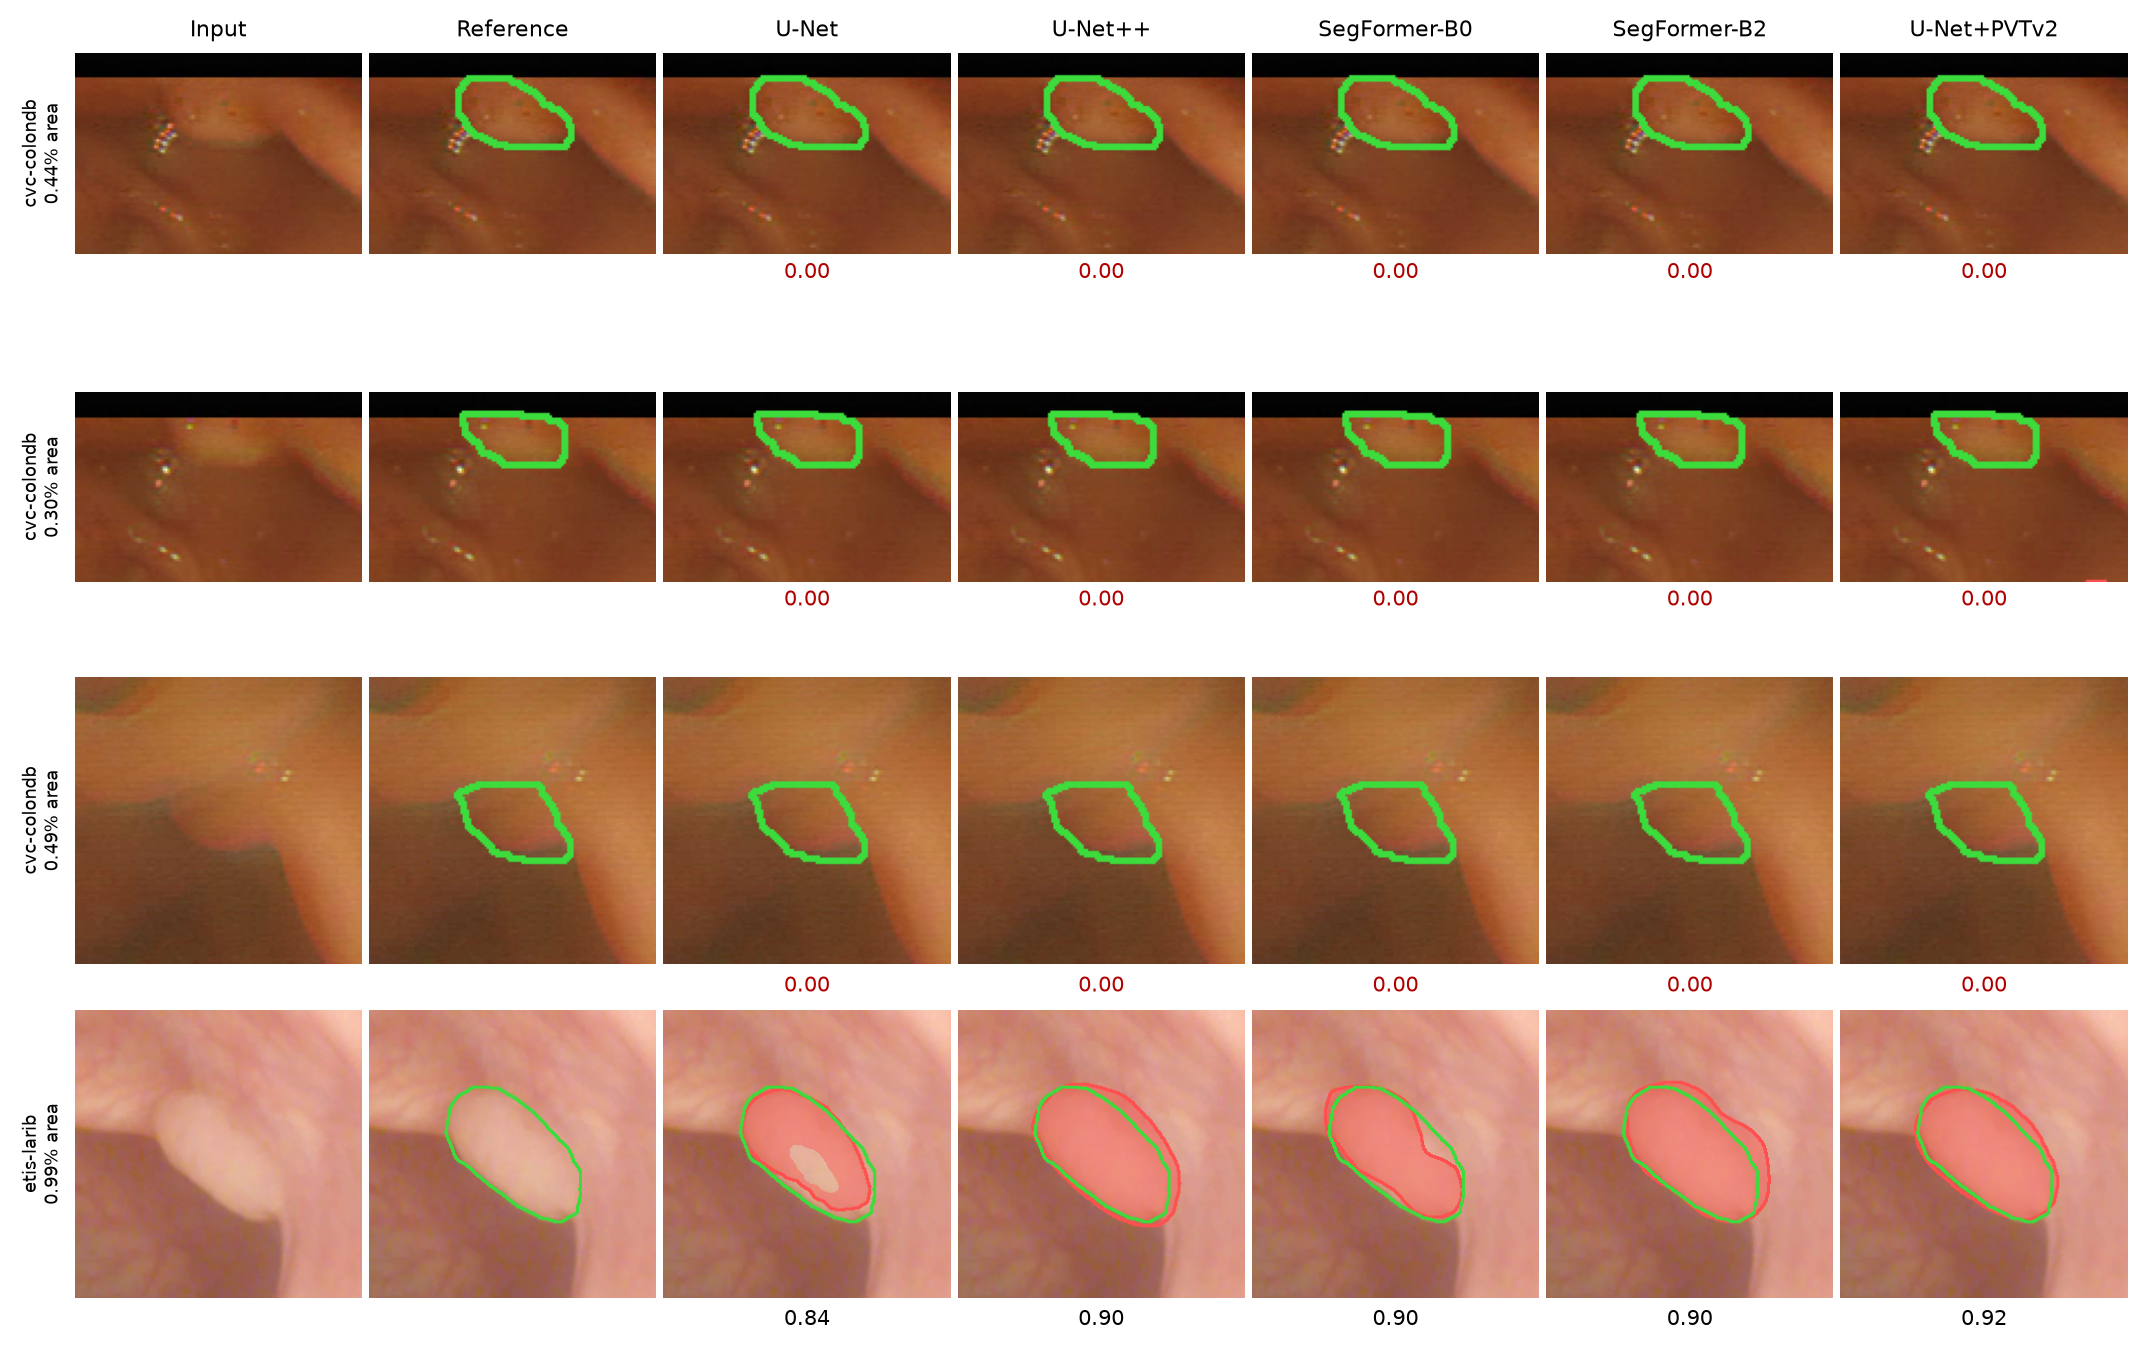
\includegraphics[width=0.96\textwidth]{f8_qualitative.pdf}
\caption{Small-lesion failures on external data, cropped around the
reference for visibility. Green contours are the reference annotation, red
overlays are predictions, and the number under each panel is Dice. Rows~1--3
show CVC-ColonDB lesions of 0.30--0.49\% of the frame for which every
architecture predicts an empty mask. Row~4 shows a 0.99\% ETIS-Larib lesion
that all five segment accurately, indicating a threshold effect rather than a
uniform difficulty. No model was trained on any image shown.}
\label{fig:qual}
\end{figure*}
Fig.~\ref{fig:qual} makes the failure mode concrete. Evaluating all
\nQualSmall\ external images whose lesion occupies under 1\% of the frame,
there are \nQualAllMiss\ (\pctQualAllMiss\%) for which \emph{no} architecture
detects the lesion at all, and \nQualZeroDice\ for which every architecture
returns an entirely empty mask. The failure is not imprecise delineation but
non-detection, and it is shared across backbone families: the same lesions
are missed by the 3.7M-parameter convolutional model and by the
28.1M-parameter transformer alike.

Larger transformer backbones mitigate but do not solve the problem: detection
on sub-1\% lesions rises from 0.44 (SegFormer-B0) to 0.59 (U-Net+PVTv2),
still far below the 0.86--0.89 achieved on large lesions.

\subsection{Flat lesions incur a consistent penalty}

Sessile (flat) lesions are segmented \sesGapLo--\sesGapHi\ Dice points worse
than non-sessile lesions, consistently across all five architectures
(Table~\ref{tab:sessile}, Fig.~\ref{fig:strata}). The penalty is not a
uniform downward shift but is driven by a tail of near-total failures.
Modern backbones reduce the gap (to \sesGapLo) without eliminating it.

\begin{table*}[t]
\centering
\footnotesize
\caption{Sessile (flat) versus non-sessile lesions, in domain. Differences are bootstrap means with 95\% percentile intervals; $p$ from a two-sided permutation test on the difference of means.}
\label{tab:sessile}
\begin{tabular}{lccc}
\toprule
Model & Sessile ($n{=}196$) & Non-sessile ($n{=}804$) & Difference \\
\midrule
U-Net & 0.8500 & 0.9131 & $-0.0632$ \\
U-Net++ & 0.8481 & 0.9140 & $-0.0660$ \\
SegFormer-B0 & 0.8305 & 0.9085 & $-0.0780$ \\
SegFormer-B2 & 0.8692 & 0.9251 & $-0.0559$ \\
U-Net+PVTv2 & 0.8693 & 0.9240 & $-0.0547$ \\
\bottomrule
\end{tabular}
\end{table*}


\begin{figure*}[t]
\centering
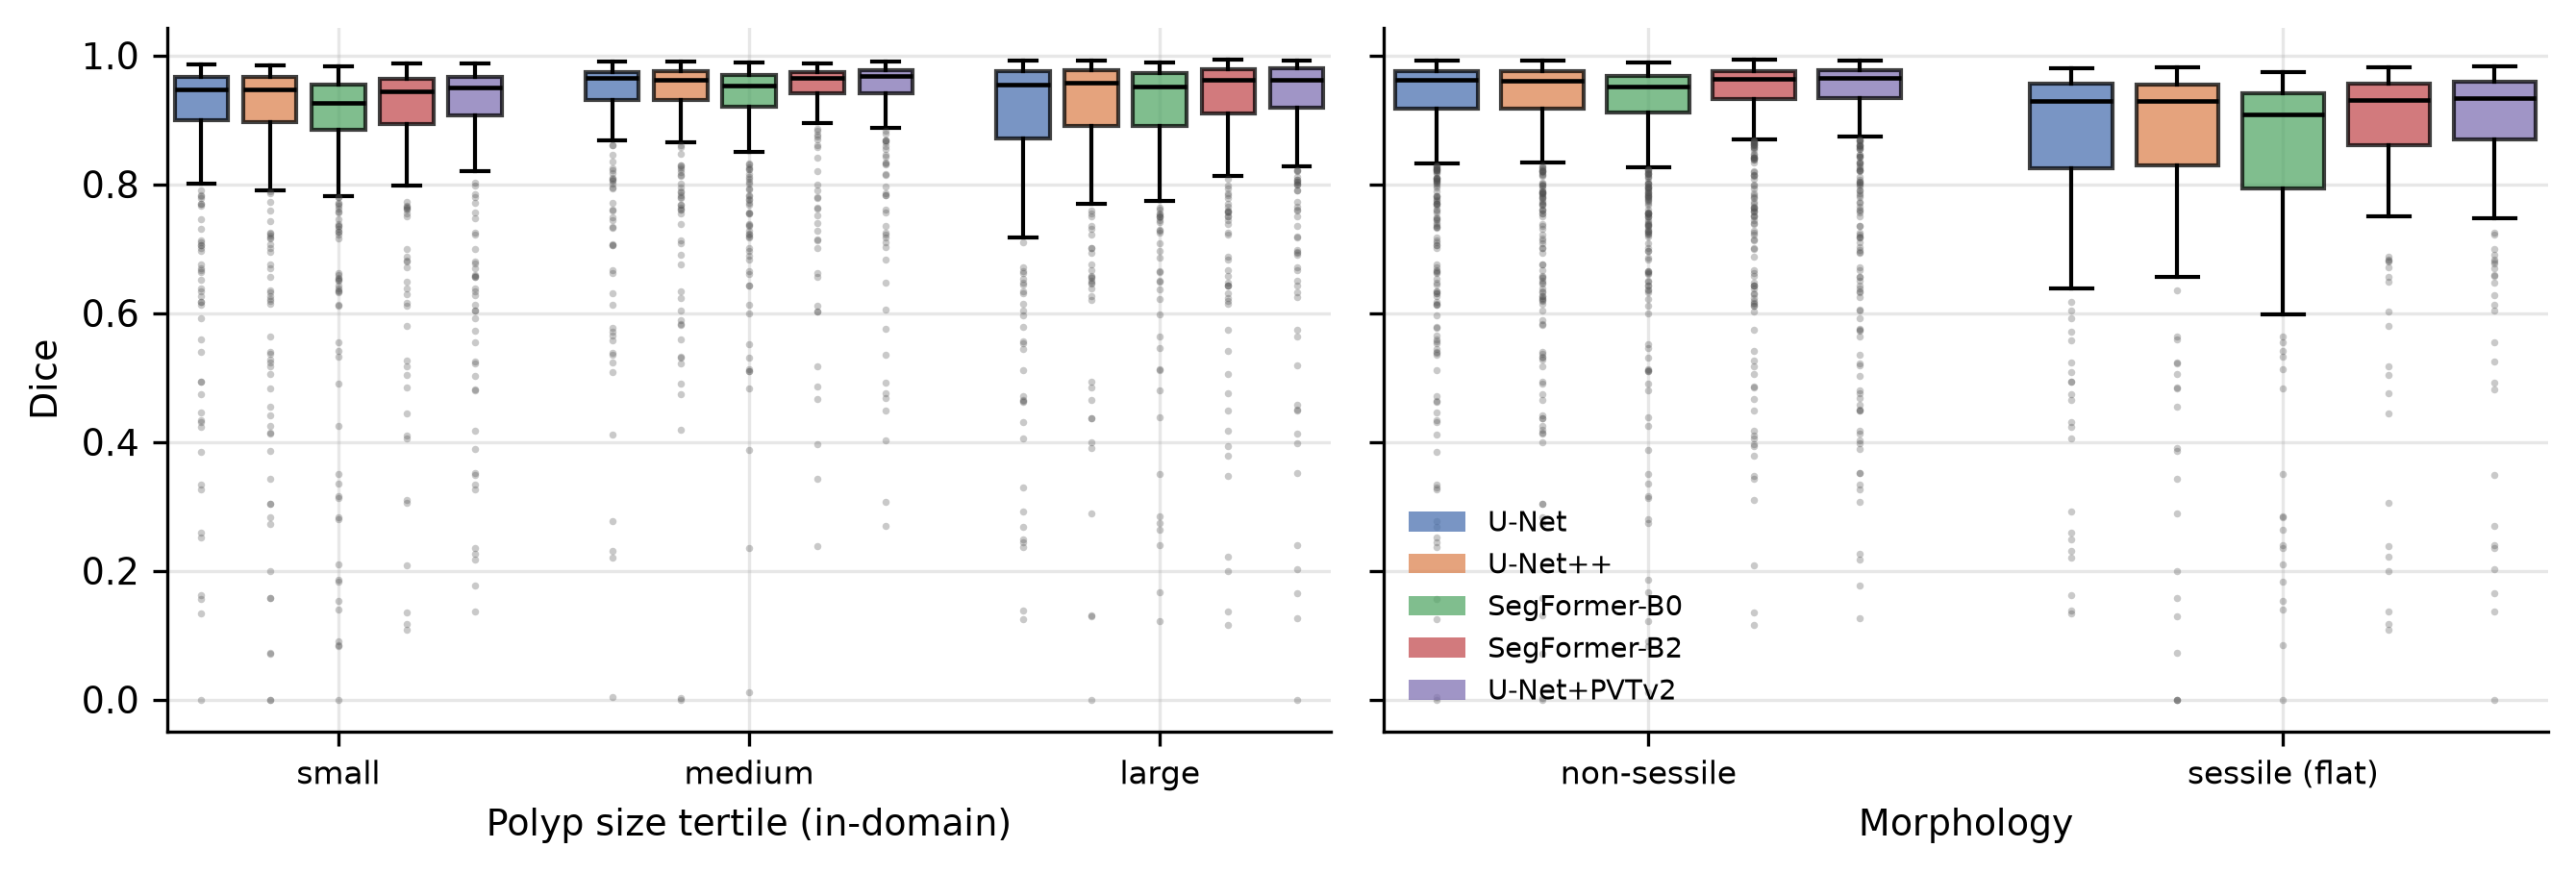
\includegraphics[width=0.92\textwidth]{f6_strata.pdf}
\caption{Per-image Dice distributions by stratum, in domain. Boxes show
quartiles, whiskers 1.5\,IQR, points are outliers. The sessile distributions
carry a pronounced lower tail that an aggregate score does not express.}
\label{fig:strata}
\end{figure*}

\subsection{A subgroup finding that did not replicate}

Before adopting cross-validation we analysed a conventional 80/10/10 split,
whose test set contains 19 sessile images. On that split U-Net++ appeared
almost unaffected by the flat-lesion penalty ($-0.002$ Dice) while U-Net and
SegFormer-B0 lost 0.061 and 0.046 respectively---an apparent architectural
robustness on the clinically hardest subgroup, and an inviting result.

It did not survive. Under five-fold cross-validation, with 196 sessile test
images, all architectures show a penalty of \sesGapLo--\sesGapHi\
(Fig.~\ref{fig:splitcv}); compared on sessile images alone, U-Net++ is not
significantly better than U-Net. The single-split confidence interval for
U-Net's penalty spans 0.112 Dice, wide enough to accommodate almost any
conclusion. We report this because it is the same error the field's standard
protocol invites, and because we made it ourselves.

\begin{figure}[t]
\centering
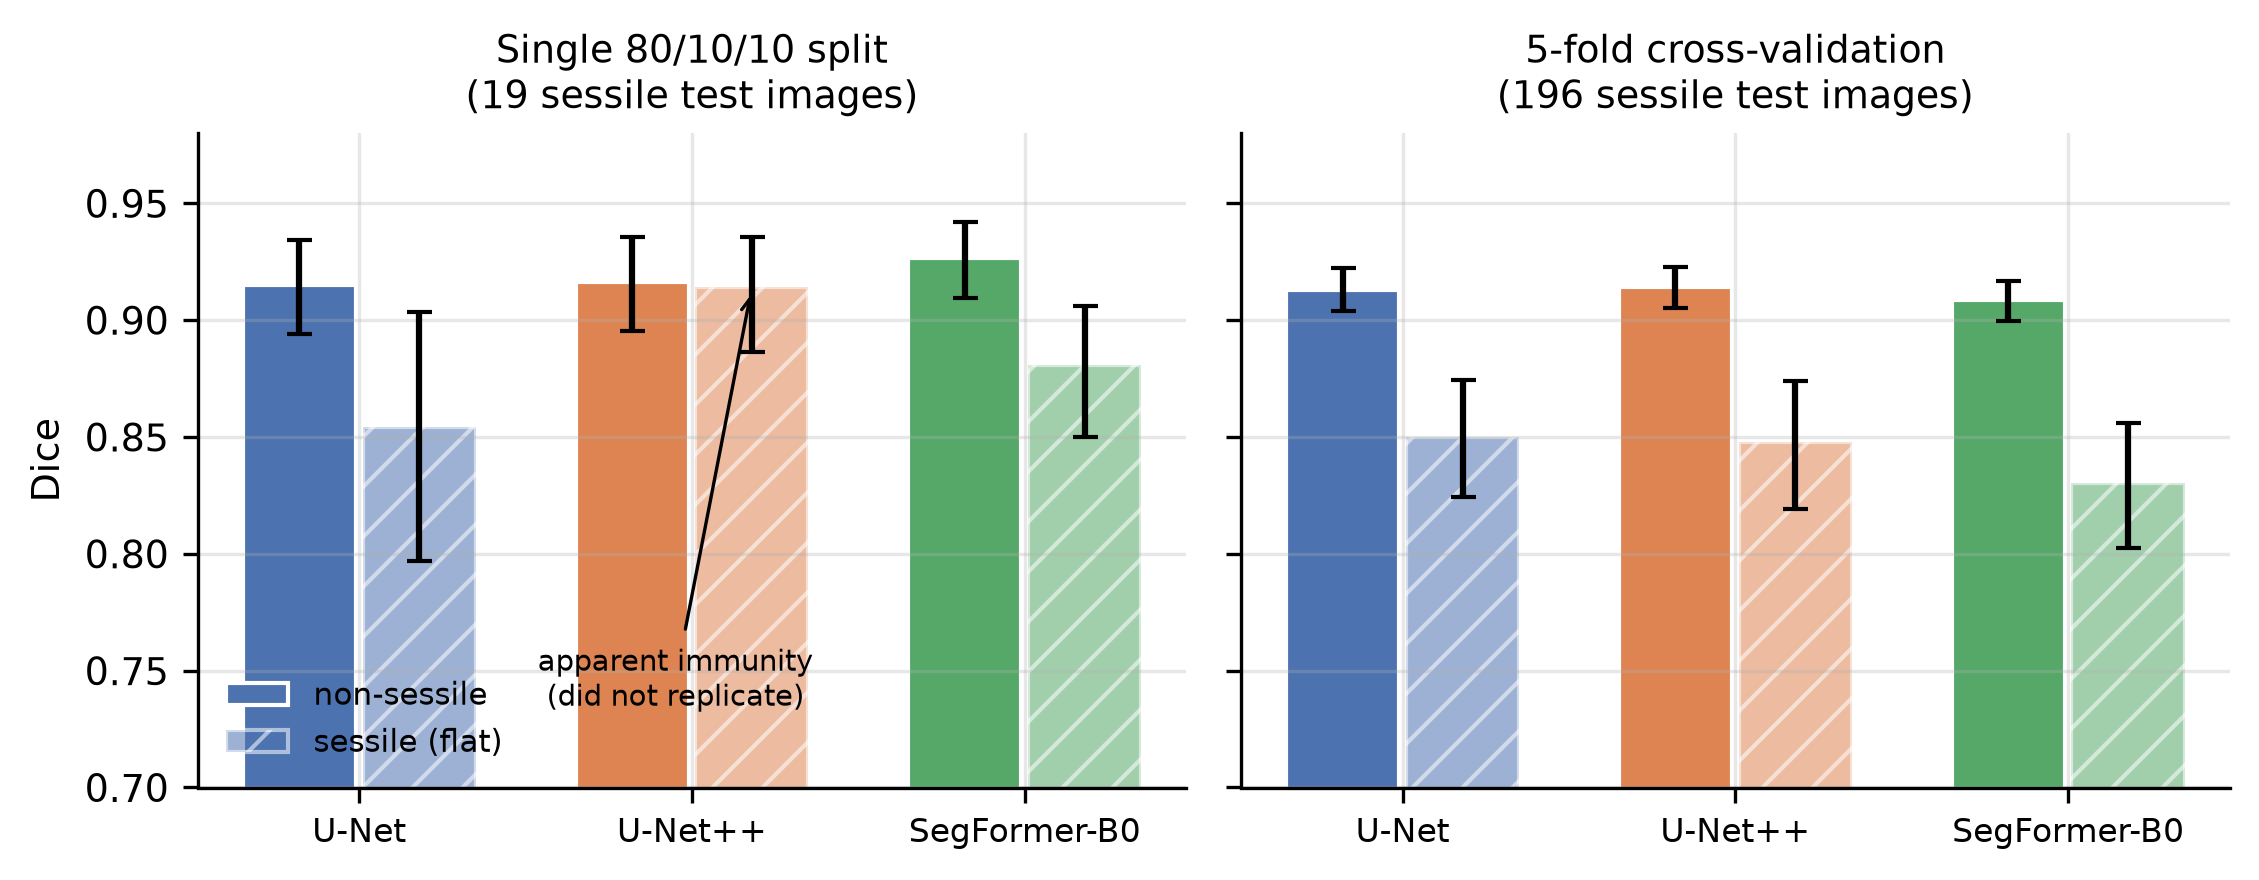
\includegraphics[width=\columnwidth]{f4_split_vs_cv.pdf}
\caption{The sessile penalty measured two ways. With 19 sessile test images
(left) U-Net++ appears unaffected; with 196 (right) all architectures show a
consistent penalty. Error bars are bootstrap 95\% confidence intervals.}
\label{fig:splitcv}
\end{figure}

\subsection{The noise floor exceeds many reported differences}

To determine which differences are meaningful we measured the variance of the
protocol itself. Each architecture was trained three times with an identical
command, seed, fold and dataset; any resulting spread is implementation
non-determinism rather than a modelling effect.

The mean within-configuration standard deviation is
$\sigma_{\mathrm{run}}=\sigmarun$ Dice, with spreads up to 0.017
(Table~\ref{tab:variance}). Against this floor, \nBelowNoise\ of
\nPairsTotal\ pairwise in-domain architecture comparisons are unresolvable,
including U-Net versus U-Net++ ($0.1\sigma_{\mathrm{run}}$) and SegFormer-B2
versus U-Net+PVTv2 ($0.2\sigma_{\mathrm{run}}$). Notably, a paired
significance test over 1000 images certifies far smaller differences as
``highly significant''; statistical significance at this sample size is not
evidence of a reproducible difference.

\begin{table*}[t]
\centering
\footnotesize
\caption{Test-Dice spread across repeated runs of an identical configuration (same seed, same fold, same data). Neither seeding the data-loader RNGs nor enabling deterministic CUDA kernels removes the variance.}
\label{tab:variance}
\begin{tabular}{llccc}
\toprule
Cond. & Configuration & Mean sd & Mean spread & Max spread \\
\midrule
A & unfixed worker RNG, default kernels & 0.0058 & 0.0108 & 0.0174 \\
B & unfixed worker RNG, deterministic & 0.0046 & 0.0065 & 0.0082 \\
C & fixed worker RNG, default kernels & 0.0056 & 0.0107 & 0.0154 \\
D & fixed worker RNG, deterministic & 0.0046 & 0.0088 & 0.0188 \\
\bottomrule
\end{tabular}
\end{table*}


\subsection{The variance comes from checkpoint selection, not from seeds}

We expected data-pipeline randomness or non-deterministic CUDA kernels. Both
hypotheses failed. Seeding all data-loader worker RNGs left the mean spread
unchanged (0.0108 to 0.0107), and additionally enabling deterministic kernels
reduced it only to 0.0088 (Table~\ref{tab:variance}, Fig.~\ref{fig:selection}).

The actual mechanism is model selection. Across \nPairs\ pairs of identical
runs, the epoch selected as ``best'' by validation Dice differs by
\meanDeltaEpoch\ epochs on average, and the divergence in test Dice scales
with that difference ($r=\rEpochTest$): pairs selecting epochs within 5 of one
another differ by \dTestClose\ Dice, while pairs 15 or more apart differ by
\dTestFar. Meanwhile the difference in validation Dice is uninformative about
the difference in test Dice ($r=\rValTest$). Because the validation curve is
flat near its maximum---in one case identical runs chose epochs 19, 19 and 40
while validation Dice differed by 0.0003---the argmax is close to arbitrary,
and infinitesimal numerical differences select materially different models.

\begin{figure*}[t]
\centering
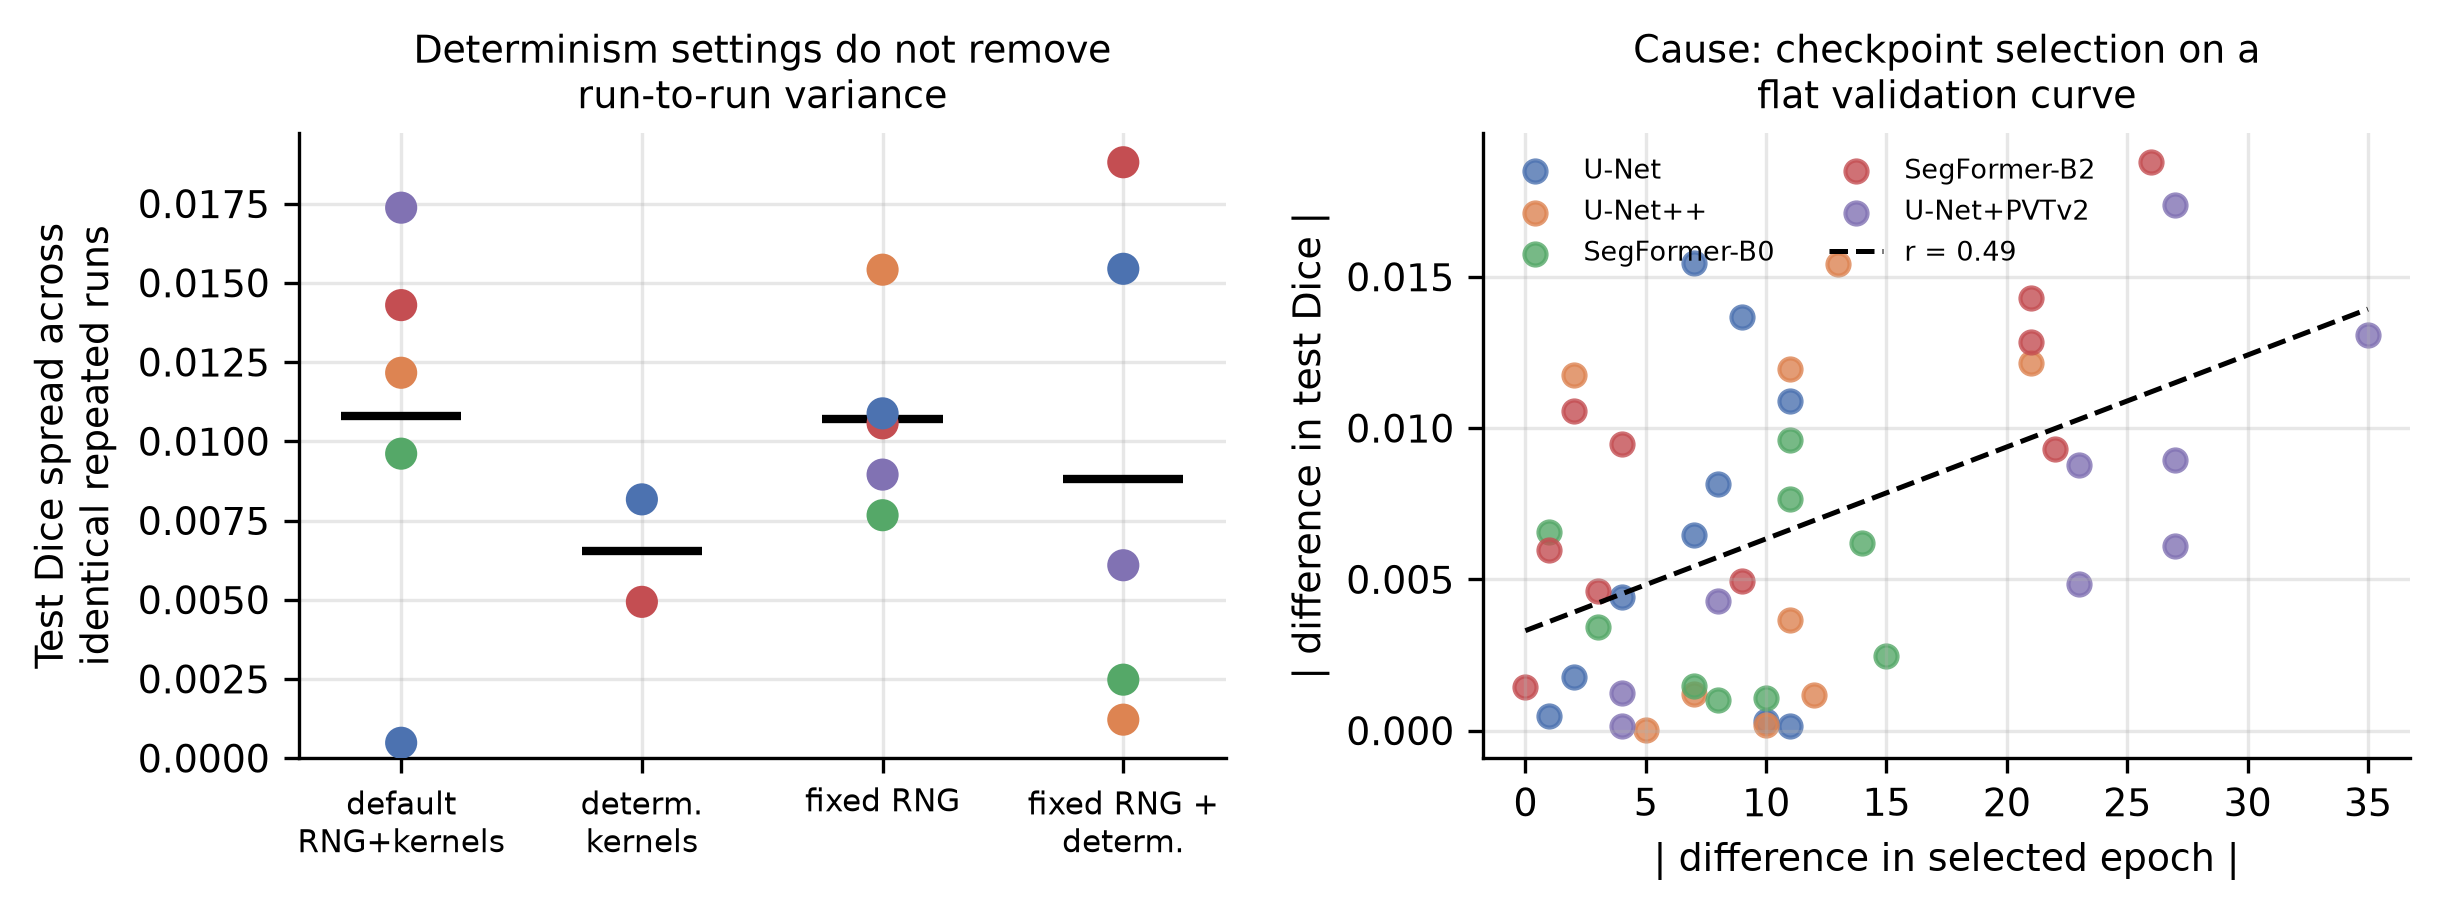
\includegraphics[width=0.92\textwidth]{f3_selection.pdf}
\caption{Left: spread in test Dice across repeated identical runs under four
determinism configurations; horizontal bars are means over architectures.
Right: the divergence in test Dice grows with the difference in selected
epoch.}
\label{fig:selection}
\end{figure*}

\subsection{Cross-dataset evaluation resolves what in-domain evaluation cannot}

All architectures degrade under domain shift, from 0.89--0.91 in domain to
\worstEtis--\bestEtis\ on ETIS-Larib (Table~\ref{tab:cross},
Fig.~\ref{fig:cross}). More useful than the degradation itself is what it
does to discrimination. Expressed in units of the measured noise floor, the
spread between best and worst architecture is \sigmaInDomain$\sigma$ in
domain but \sigmaEtis$\sigma$ on ETIS-Larib (Table~\ref{tab:resolving},
Fig.~\ref{fig:resolving}). Architectures that in-domain evaluation cannot
separate differ by 0.116 Dice out of domain.

\begin{table*}[t]
\centering
\footnotesize
\caption{Zero-shot transfer. Models are trained on Kvasir-SEG only; each value is the mean over the five cross-validation fold models. Upper block: Dice. Lower block: per-lesion detection rate at IoU $\geq 0.5$.}
\label{tab:cross}
\begin{tabular}{lccccc}
\toprule
Model & Kvasir-\allowbreak SEG & CVC-\allowbreak ClinicDB & CVC-\allowbreak 300 & CVC-\allowbreak ColonDB & ETIS-\allowbreak Larib \\
\midrule
\multicolumn{6}{l}{\emph{Dice}}\\
\quad U-Net & 0.9007 & 0.8489 & 0.8552 & 0.7191 & 0.6805 \\
\quad U-Net++ & 0.9011 & 0.8535 & 0.8443 & 0.7250 & 0.6551 \\
\quad SegFormer-B0 & 0.8932 & 0.8450 & 0.8395 & 0.7275 & 0.6743 \\
\quad SegFormer-B2 & 0.9142 & 0.8718 & 0.8550 & 0.7738 & 0.7685 \\
\quad U-Net+PVTv2 & 0.9133 & 0.8738 & 0.8728 & 0.7668 & 0.7706 \\
\midrule
\multicolumn{6}{l}{\emph{Per-lesion detection rate}}\\
\quad U-Net & 0.9308 & 0.8879 & 0.8867 & 0.7632 & 0.7361 \\
\quad U-Net++ & 0.9328 & 0.8920 & 0.8867 & 0.7742 & 0.7262 \\
\quad SegFormer-B0 & 0.9269 & 0.8850 & 0.8900 & 0.7589 & 0.7207 \\
\quad SegFormer-B2 & 0.9408 & 0.9151 & 0.8867 & 0.8132 & 0.8129 \\
\quad U-Net+PVTv2 & 0.9334 & 0.9139 & 0.8933 & 0.8147 & 0.8279 \\
\bottomrule
\end{tabular}
\end{table*}

\begin{table*}[t]
\centering
\footnotesize
\caption{Resolving power of each test set. The spread is the Dice difference between the best and worst of the five architectures; $\sigma_{\mathrm{run}}$ is the measured run-to-run standard deviation. A test set can only distinguish architectures whose gaps exceed this noise floor.}
\label{tab:resolving}
\begin{tabular}{lccll}
\toprule
Test set & Spread & $/\sigma_{\mathrm{run}}$ & Best & Worst \\
\midrule
Kvasir-SEG & 0.0210 & 3.9 & SegFormer-B2 & SegFormer-B0 \\
CVC-ClinicDB & 0.0287 & 5.4 & U-Net+PVTv2 & SegFormer-B0 \\
CVC-300 & 0.0333 & 6.2 & U-Net+PVTv2 & SegFormer-B0 \\
CVC-ColonDB & 0.0548 & 10.3 & SegFormer-B2 & U-Net \\
ETIS-Larib & 0.1155 & 21.6 & U-Net+PVTv2 & U-Net++ \\
\bottomrule
\end{tabular}
\end{table*}


\begin{figure}[t]
\centering
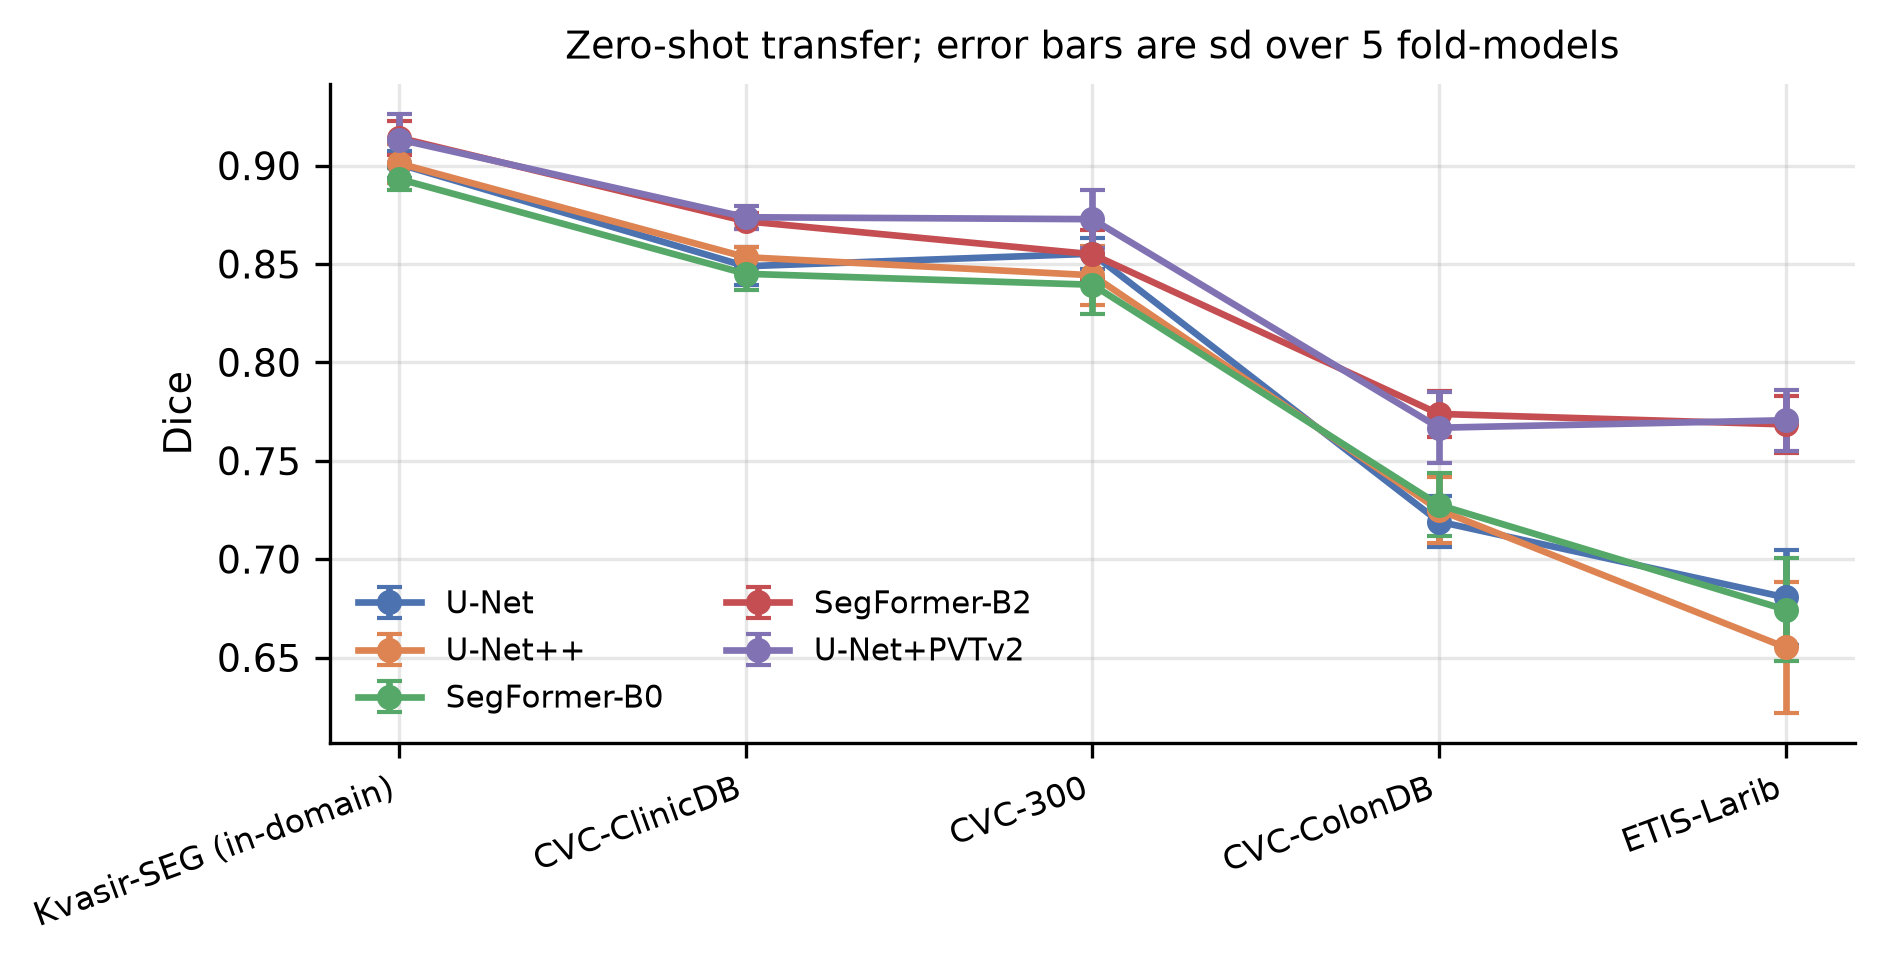
\includegraphics[width=\columnwidth]{f5_cross_dataset.pdf}
\caption{Zero-shot transfer from Kvasir-SEG. Error bars are standard
deviations over the five cross-validation fold models.}
\label{fig:cross}
\end{figure}

\begin{figure}[t]
\centering
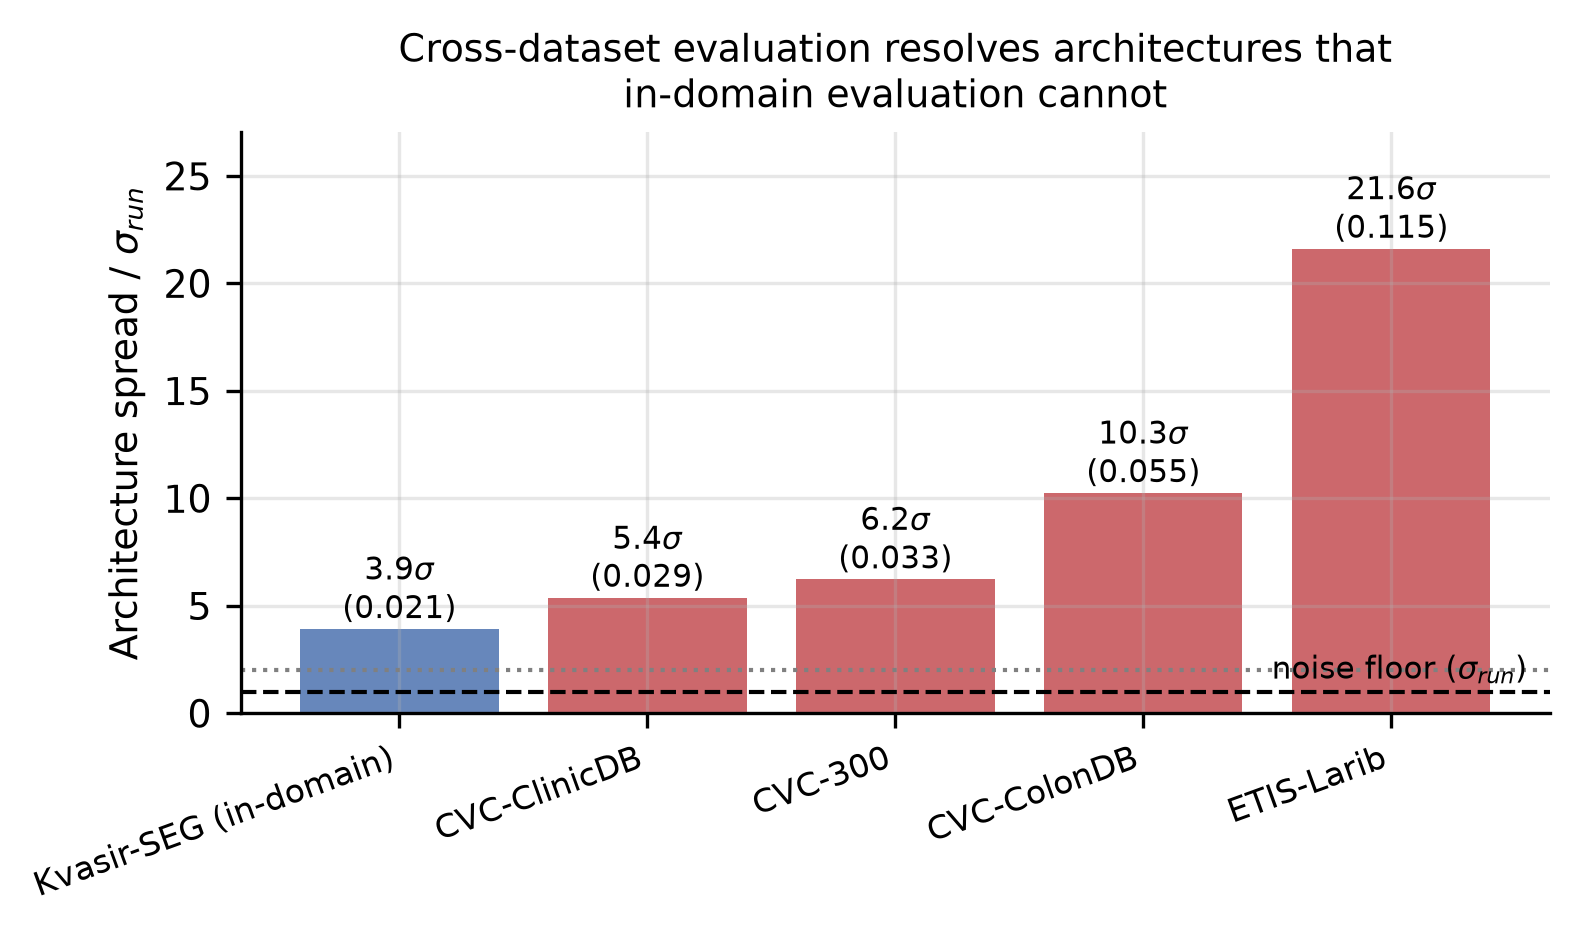
\includegraphics[width=\columnwidth]{f2_resolving.pdf}
\caption{Architecture spread on each test set, expressed in units of the
measured run-to-run noise floor $\sigma_{\mathrm{run}}$.}
\label{fig:resolving}
\end{figure}

Flip test-time augmentation improves Dice by \ttaIn\ in domain and \ttaOut\
out of domain, roughly twice as much, suggesting that part of the transfer
gap reflects sensitivity to nuisance transformations rather than irreducible
domain difference.

\subsection{Region overlap understates multifocal failure}

Region-overlap metrics score an image as a single region. An image containing
ten lesions of which nine are missed is penalised only in proportion to their
combined area: in a constructed example, missing two of three lesions costs
just 8.3 Dice points while per-lesion detection correctly reports 33\%. We
observed this in practice on a test image containing ten distinct lesions,
almost none of which were recovered by any architecture, at a Dice cost that
did not reflect the clinical failure. Per-lesion detection rates should
accompany overlap metrics whenever multifocal images are present.

\section{Discussion}

Three practical conclusions follow.

\smallskip\noindent\textbf{Benchmark on lesions that resemble the clinical problem.}\ 
Kvasir-SEG's lesions are large: a median of \kvasirMedianArea\% of the frame,
with \nSmallKvasir\ images below 1\%. Because detection collapses precisely
in the range the benchmark lacks, in-domain scores are close to uninformative
about the clinically decisive regime. Datasets such as CVC-ColonDB and
ETIS-Larib should be part of routine evaluation, not an optional extra.

\smallskip\noindent\textbf{Report a noise floor, and compare against it.}\ 
Differences below $\sigma_{\mathrm{run}}$ should not be interpreted, however
significant a paired test declares them. Measuring the floor costs a handful
of repeated runs. Because the dominant source is checkpoint selection rather
than kernel non-determinism, the mitigations are procedural: average weights
over the final epochs, select on a smoothed validation criterion, use larger
validation sets, or report the mean of repeated runs. Fixing a seed is not
sufficient, and---as our own results show---neither is enabling deterministic
kernels.

\smallskip\noindent\textbf{Prefer test sets with resolving power.}\ 
If the purpose of a benchmark is to rank methods, its value depends on the
ratio between the differences it exposes and the noise it carries. On that
criterion ETIS-Larib is roughly five times more informative than in-domain
Kvasir-SEG, despite---indeed because of---being harder and further from the
training distribution.

\subsection{Limitations}

Kvasir-SEG provides no patient identifiers, so splits are image-level and
frames from one procedure may co-occur across folds; this affects both
protocols we compare and does not bear on the replication argument. Our
size strata use relative lesion area rather than physical size, which the
datasets do not record. The repeat study uses three runs per configuration on
one fold, so per-architecture variance estimates are themselves uncertain,
and it was conducted on a single GPU model; we separately observed that
re-running the full cross-validation on different hardware shifted mean Dice
by up to 0.005, suggesting the cross-hardware floor is no smaller. We did not
retrain specialised polyp architectures such as PraNet or Polyp-PVT:
reproducing them faithfully under a different recipe risks understating them,
so we instead span their backbone families under one controlled recipe. All
results are on curated still frames and do not establish clinical utility,
which requires prospective video evaluation.

\section{Methods}

\smallskip\noindent\textbf{Data.}\  Kvasir-SEG \cite{jha2020kvasirseg} provides 1000
colonoscopy images with expert masks at resolutions from $332\times487$ to
$1920\times1072$. The Kvasir-Sessile subset identifies 196 flat lesions,
used here as a difficulty label rather than as additional data. External
test sets, used only for evaluation, are CVC-ClinicDB
\cite{bernal2015} (612 images), CVC-ColonDB (380), ETIS-LaribPolypDB (196)
and CVC-300 (60), obtained from the standard benchmark distribution. We
excluded that distribution's Kvasir subset, which overlaps our training data.

\smallskip\noindent\textbf{Architectures.}\  U-Net \cite{ronneberger2015} and U-Net++
\cite{zhou2018} with ResNet-34 encoders; SegFormer-B0 and SegFormer-B2
\cite{xie2021segformer}; and a U-Net decoder over a PVTv2-B2 backbone
\cite{wang2022pvtv2}, the family used by recent specialised polyp networks.
All use ImageNet-pretrained encoders and an identical training recipe, so
architecture is the only varied factor.

\smallskip\noindent\textbf{Training.}\  Images are resized to $352\times352$. AdamW
(lr $10^{-4}$, weight decay $10^{-4}$), cosine annealing, batch size 16, up
to 60 epochs with early stopping (patience 15) on validation Dice, and an
equally weighted Dice+BCE objective. Augmentation comprises flips, affine
transforms, colour jitter, blur and noise. Mixed precision (bfloat16) is used
throughout. Experiments ran on a single NVIDIA RTX 4090.

\smallskip\noindent\textbf{Cross-validation.}\  Five folds stratified jointly on size tertile
and sessile status; each fold uses 700 training, 100 validation and 200 test
images, so every image is tested exactly once. Pooled strata therefore
contain approximately 333 images per size tertile and 196 sessile images.

\smallskip\noindent\textbf{Metrics.}\  Predictions are resized to native resolution before
scoring. We report Dice, IoU, Boundary-F1 and HD95. Boundary tolerance is set
to 0.5\% of the image diagonal rather than a fixed pixel count, because
predictions made at a fixed network resolution and upsampled to images
differing five-fold in diagonal are not otherwise comparable; using a fixed
2\,px tolerance depresses Boundary-F1 from 0.67 to 0.48 for U-Net, an
artefact of resolution. Per-lesion detection matches ground-truth connected
components against predicted components at IoU $\geq 0.5$, discarding
components below 0.02\% of the image as noise.

\smallskip\noindent\textbf{Statistics.}\  Architecture comparisons use the Wilcoxon signed-rank
test paired over per-image Dice with Holm correction. Stratum contrasts use
two-sided permutation tests on the difference of means with percentile
bootstrap intervals (10\,000 resamples), so that interval and $p$-value refer
to the same estimand; a rank-based test disagrees with a mean-difference
interval on these skewed distributions.

\smallskip\noindent\textbf{Variance study.}\  Each architecture was trained three times on fold
0 with identical arguments under four configurations: default RNG and
kernels; deterministic kernels only; seeded data-loader workers only; and
both. $\sigma_{\mathrm{run}}$ is the mean within-configuration standard
deviation of test Dice.

\section*{Ethics statement}

This study used only publicly available, fully de-identified image datasets
released for research use by their original providers. No new patient data
were collected and no human participants were involved, so institutional
ethics approval was not required. Use of Kvasir-SEG is restricted to research
and educational purposes under its licence.

\section*{Competing interests}

% Replace with the accurate wording once employer clearance is resolved.
The author is employed as a software engineer by Karl Storz Endoscopy. The
company had no role in the conception, design, execution, analysis or
reporting of this study, provided no funding or resources for it, and the
work uses exclusively publicly available datasets and open-source software.
The author declares no other competing interests.

\section*{Data and code availability}

Code, cross-validation splits and per-image results for all 88 training runs
are available at
\url{https://github.com/rishitpuri/polyp-segmentation-evaluation} and archived at Zenodo
(\url{https://doi.org/10.5281/zenodo.22841360}). The datasets are available
from their original providers; Kvasir-SEG is restricted to research and
educational use.

\section*{Author contributions}

R.P. conceived the study, implemented the experiments, performed the
analysis, and wrote the manuscript.

\begin{thebibliography}{99}

\bibitem{leufkens2012}
A.~M. Leufkens, M.~G. van Oijen, F.~P. Vleggaar, and P.~D. Siersema.
Factors influencing the miss rate of polyps in a back-to-back colonoscopy
study. \emph{Endoscopy}, 44(5):470--475, 2012.

\bibitem{vanrijn2006}
J.~C. van Rijn et al.
Polyp miss rate determined by tandem colonoscopy: a systematic review.
\emph{American Journal of Gastroenterology}, 101(2):343--350, 2006.

\bibitem{jha2020kvasirseg}
D.~Jha et al.
Kvasir-SEG: A segmented polyp dataset.
In \emph{International Conference on Multimedia Modeling}, 451--462, 2020.

\bibitem{bernal2015}
J.~Bernal et al.
WM-DOVA maps for accurate polyp highlighting in colonoscopy.
\emph{Computerized Medical Imaging and Graphics}, 43:99--111, 2015.

\bibitem{ronneberger2015}
O.~Ronneberger, P.~Fischer, and T.~Brox.
U-Net: Convolutional networks for biomedical image segmentation.
In \emph{MICCAI}, 234--241, 2015.

\bibitem{zhou2018}
Z.~Zhou, M.~M.~R. Siddiquee, N.~Tajbakhsh, and J.~Liang.
UNet++: A nested U-Net architecture for medical image segmentation.
In \emph{DLMIA}, 3--11, 2018.

\bibitem{xie2021segformer}
E.~Xie et al.
SegFormer: Simple and efficient design for semantic segmentation with
transformers. In \emph{NeurIPS}, 2021.

\bibitem{wang2022pvtv2}
W.~Wang et al.
PVT v2: Improved baselines with pyramid vision transformer.
\emph{Computational Visual Media}, 8(3):415--424, 2022.

\bibitem{fan2020pranet}
D.-P. Fan et al.
PraNet: Parallel reverse attention network for polyp segmentation.
In \emph{MICCAI}, 263--273, 2020.

\bibitem{cheng2021boundaryiou}
B.~Cheng, R.~Girshick, P.~Doll\'ar, A.~C. Berg, and A.~Kirillov.
Boundary IoU: Improving object-centric image segmentation evaluation.
In \emph{CVPR}, 15334--15342, 2021.

\bibitem{maierhein2024metrics}
L.~Maier-Hein et al.
Metrics reloaded: Recommendations for image analysis validation.
\emph{Nature Methods}, 21:195--212, 2024.

\bibitem{varoquaux2018}
G.~Varoquaux.
Cross-validation failure: Small sample sizes lead to large error bars.
\emph{NeuroImage}, 180:68--77, 2018.

\bibitem{picard2021}
D.~Picard.
Torch.manual\_seed(3407) is all you need: On the influence of random seeds in
deep learning architectures for computer vision.
\emph{arXiv:2109.08203}, 2021.

\end{thebibliography}

\end{document}
